\begin{figure}[htbp]
\centering
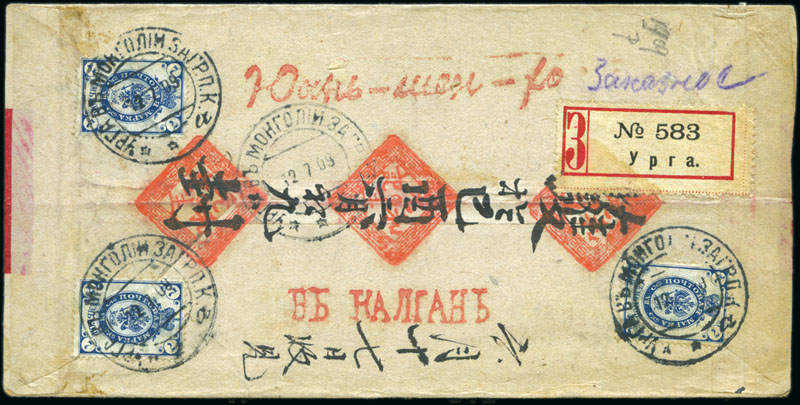
\includegraphics[width=.95\textwidth]{../russian-post-in-mongolia/10138.jpg}
\caption{ 
10138 URGA: 1909 Native cover sent registered to Kalgan, franked with 
three Russia Arms 7k paying double the rate plus registration, 
tied by Urga 12.7.09 type 6 cds in blue-black, registration label 
adjacent (Hellrigl type 8 rated R), Kalgan type 3 arrival cds, fine and 
scarce registered cover.
\euro 1,500.00 
} 
\end{figure}   

\begin{figure}[htbp]
\centering
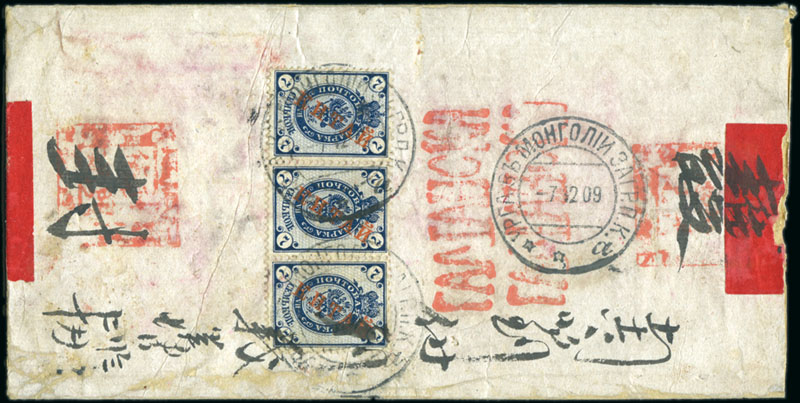
\includegraphics[width=.95\textwidth]{../russian-post-in-mongolia/10139.jpg}
\caption{ 
10139 URGA: 1909 Native cover sent to Kalgan franked with strip of three 
Russia Arms 7k "KITAI", tied by Urga 7.12.09 type 6 cds, with Kalgan type 3
arrival cds on reverse, fine and rare usage of these overprinted stamps that
were not for sale in the Mongolian Offices.

Provenance: Ex Tolman
\euro 2,000.00 
} 
\end{figure}  


\begin{figure}[htbp]
\centering
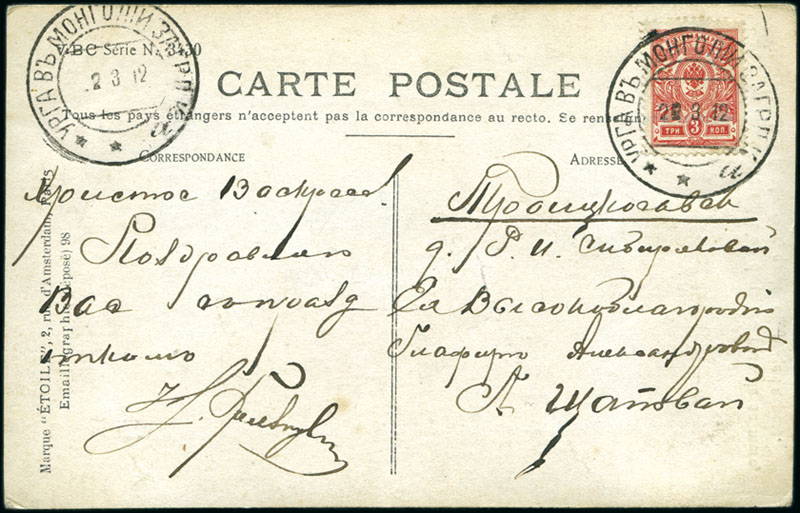
\includegraphics[width=.95\textwidth]{../russian-post-in-mongolia/10140.jpg}
\caption{ 
10140URGA: 1912 Postcard to Troitskosavsk (Siberia), with 3k red paying
the postcard rate, tied by Urga 22.3.12 type 6 cds, very fine and scarce rate.
\euro150.00 
} 
\end{figure}  

\begin{figure}[htbp]
\centering
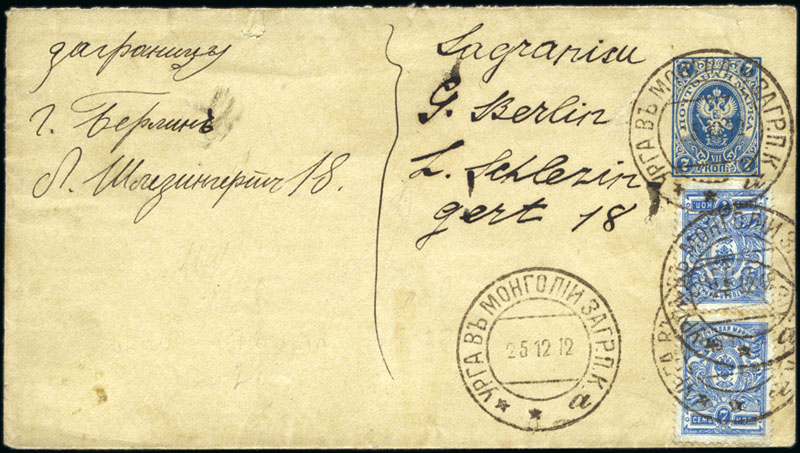
\includegraphics[width=.95\textwidth]{../russian-post-in-mongolia/10141.jpg}
\caption{ 
10141 URGA: 1912 7k Postal stationery envelope sent to Berlin, 
uprated with two 7k blue, paying double the foreign letter rate 
(overpaid 1k), all cancelled by Urga 25.12.12 type 5 cds, fine 
and rare usage of stationery
\euro 300.00 
} 
\end{figure} 

\begin{figure}[htbp]
\centering
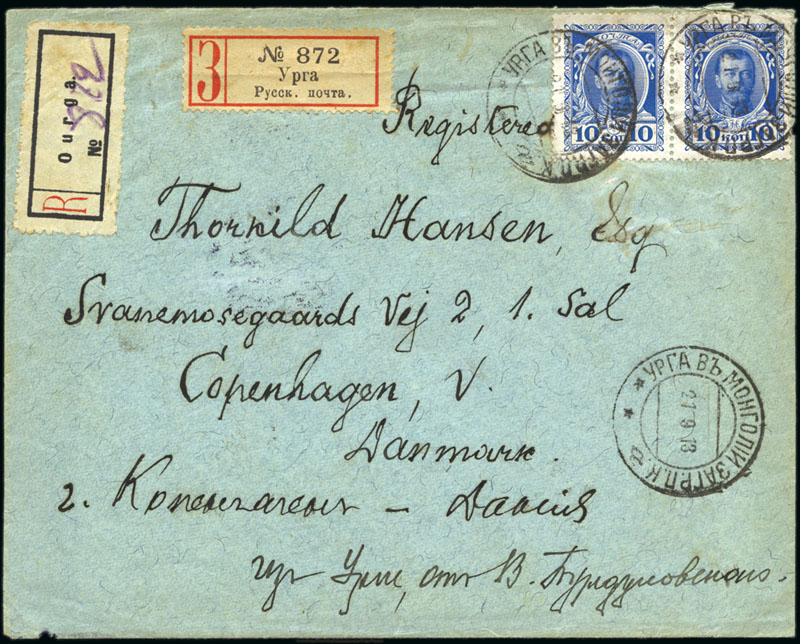
\includegraphics[width=.95\textwidth]{../russian-post-in-mongolia/10142.jpg}
\caption{ 
10142URGA: 1913 Envelope sent registered to Copenhagen, with 10k Romanov pair
tied by Urga 21.9.13 type 6 cds, paying the single foreign rate plus
registration, with Russian reg'n label (Hellrigl type 9 rated RR) and reg'n
label in French (type 13 rated RR) adjacent, a rare destination and only two
covers and a card known with two reg'n labels according to 
"The Postal History of Mongolia" pg.7 by Hellrigl. Plus Tchilinghirian
states that "Romanov stamps are of great rarity with Urga cancellations",
and is one of only 7 covers recorded by Hellrigl)
\euro 3,000.00 
} 
\end{figure}  

\begin{figure}[htbp]
\centering
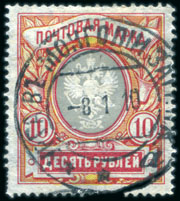
\includegraphics[width=.35\textwidth]{../russian-post-in-mongolia/10143.jpg}
\caption{ 
10143 URGA: Four stamps with the Urga type 6 cds incl. piece with a pair of the
1909-12 10k blue, plus single 1906 10R and 1913 50k Romanov (both with trimmed perfs)
Currently (SAN)...\euro 100.00 
} 
\end{figure}  

\begin{figure}[htbp]
\centering
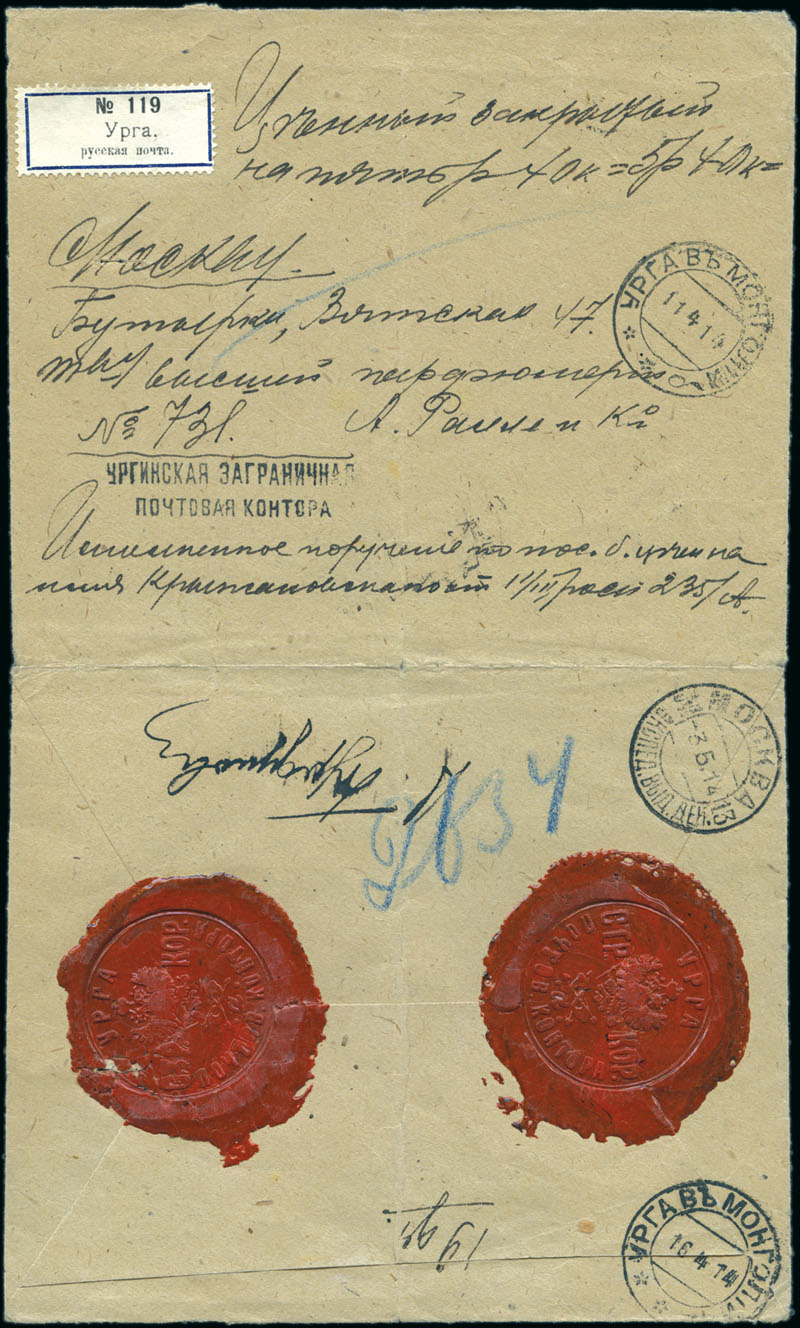
\includegraphics[width=.95\textwidth]{../russian-post-in-mongolia/10144.jpg}
\caption{ 
10144 URGA: 1914 Insured Money Letter to Moscow, cancelled by Urga 11.4.14 type 7A 
cds, with registration label (Hellrigl rated RRR, believed to be unique) 
and previously unrecorded "Urga Post Office Abroad" two line 
Cyrillic hs adjacent, reverse with two large wax seals inscribed 
"Urga Post Office / Insured Correspondence" also previously unrecorded
and a rare Moscow "Expeditsia" cds for forwarding money, opened for display,
possibly unique.
Provenance: Ex Tolman
\euro 2,000.00
} 
\end{figure}  













              